% !TeX spellcheck = en_GB
\section{Overview of technologies}\label{Overview}
Before we start going into detail about how to work with Hibernate Search in a generic environment, we will give a short overview of relevant technologies first. We will explain why ORMs in general and the JPA specification in particular are beneficial. Then, we will explain what fulltext search engines are used for and give a short overview about the available solutions for Java. We will see that generalizing Hibernate Search for any JPA implementation is a good approach and that it has benefits over using the different search solutions available.

\subsection{Object Relational Mappers}
Nowadays, many popular languages like Java, C\#, etc. are object-oriented\footnote{Wikipedia on Object Oriented Programming (OOP), see~\cite{object_oriented_programming_wiki}}.
While SQL solutions for querying relational databases exist for these languages (JDBC for Java\footnote{Oracle JDBC overview, see~\cite{jdbc_oracle}}, OleDb for C\#\footnote{OleDb usage page, see~\cite{oledb_ms}}), the user either has to work with the rowsets manually or convert them into custom data transfer objects (DTO) to gain at least some "real" objects to work with. Both approaches don't suit the object oriented paradigm well as SQL "flattens" the data into rows with when querying while a well designed class model would work with multiple classes in a hierarchy.
\\
\lstset{language=sql}
\begin{lstlisting}[frame=htrbl, caption={sql query "flattening" the author and book table into rows}, label={lst:flattening.sql}]
SELECT author.id, author.name, book.id, book.name 
FROM author_book, author, author
WHERE author_book.bookid = book.id
AND author_book.authorid = author.id
\end{lstlisting}
~\\
This is where Object Relational Mappers (ORM) come into use. They map tables to entity-classes and
enable users to write queries against these classes instead of tables. The returned objects are part of a complex object hierarchy and are easier to use from a object oriented point of view.
\\
\lstset{language=java}
\begin{lstlisting}[frame=htrbl, caption={ORM query example}, label={lst:flattening.sql}]
List<Author> data = orm.query("SELECT a FROM Author a " +
	"LEFT OUTER JOIN a.books");
for(Author author : data) {
	System.out.println("name: " + author.getName() + 
		", books: " + author.getBooks());
}
\end{lstlisting}
~\\
This is especially useful if used in big software products as not all programmers have to know the exact details of the underlying database. The database system could even be completely replaced for another (provided the ORM supports the specific RDBMS), while the business logic would not changing a bit.

\subsection{JPA}

The first version of the JPA standard was released in May 2006. From then on it rose to being probably the most commonly used persistence API for Java and is considered the "industry standard approach for Object Relational Mapping"\footnote{Wikibooks on Java Persistence, see~\cite{wikibooks_on_jpa}}. While mostly known for standardizing relational database mappers (ORM), it also supports other concepts like NoSQL\footnote{Hibernate OGM project homepage, see~\cite{hibernate_ogm}} \footnote{EclipseLink project homepage, see~\cite{eclipselink}} or XML storage\footnote{EclipseLink project homepage, see~\cite{eclipselink}}. However, when talking about JPA in this thesis, we will be focusing on the relational aspects of it. Currently, the newest version of this standard is 2.1.\footnote{Wikipedia on Java Persistence API, see~\cite{wiki_jpa}}.
\\\\
Some popular relational implementations are:
\begin{itemize}
	\item Hibernate ORM (JBoss)\footnote{Hibernate ORM project homepage, see~\cite{hibernate_orm}}
	\item EclipseLink (Eclipse foundation)\footnote{EclipseLink project homepage, see~\cite{eclipselink}}
	\item OpenJPA (Apache foundation)\footnote{OpenJPA project homepage, see~\cite{openjpa}}
\end{itemize}
~\\
Using the standardized JPA API over any native ORM API has one really interesting benefit:
The specific JPA implementation can be swapped out as it comes with standards for many common use cases.
\\\\
This is particularily important if you are working in a Java EE environment. Java EE itself is a specification for platforms, mostly Web-servers (JPA is part of the Java EE spec).\footnote{Wikipedia on Java EE, see~\cite{wiki_java_ee}} Many Java EE Web-servers ship with a bundled JPA implementation that they are optimized for (Wildfly with Hibernate ORM, GlassFish with EclipseLink, ...). This means that if the server is switched, it could also be a reasonable idea to swap out the JPA implementor. If everything in the application is written in a JPA compliant way, the user will then generally not run into many problems related to this switch.

\pagebreak

\subsection{Fulltext search engines}

Conventional relational databases are good at retrieving and querying structured data. But if one wants to build a search engine atop a domain model, most RDBMS will only support the SQL-LIKE operator \footnote{w3schools on SQL LIKE, see~\cite{sql_like_w3schools}}:\\

\lstset{language=sql}
\begin{lstlisting}[frame=htrbl, caption={SQL LIKE operator in use}, label={lst:result2}]
SELECT book.id, book.name FROM book WHERE book.name LIKE %name%;
\end{lstlisting}
While this might be enough for some applications, this wildcard query doesn't support features a good search engine would need, for example:

\begin{itemize}
	\item fuzzy queries (variations of the original string will get matched, too)
	\item phrase queries (search for a specified phrase)
	\item regular expression queries (matches are determined by a regular expression)
\end{itemize}
There may exist some RDBMS that support similar query-types, but in the context of using a ORM we would then lose the ability to switch databases since, we would use vendor-specific features not every RDBMS supports.
\\\\
Fulltext search engines can be used to complement databases in this regard. They are generally not intended to be replacing the database, but add additional functionality by indexing the data that is to be searched in a more sophisticated way. We will now take a look at some of the most popular available options for Java developers (including Hibernate Search) focusing on their usage and features. After that we will give the reasoning behind why a \textbf{generic} Hibernate Search is a good idea.

\pagebreak

\subsubsection{Lucene}

\textcolor{red}{mention current version for each of these?}

\begin{quote}
	Apache Lucene™ is a high-performance, full-featured text search engine library written entirely in Java. It is a technology suitable for nearly any application that requires full-text search, especially cross-platform.\footnote{official Lucene website, see~\cite{lucene_apache_org}}
\end{quote}
Lucene serves as the basis for many fulltext search engines written in Java. It has many different utilties and modules aimed at search engine developers. However, it can be used on its own as well.

\paragraph{Concepts}

As Lucene's focus is not on storing relational data, it comes with its own set of concepts. Following is a short overview over the most important ones. These are not only the basis for Lucene, but also for the other search engines we will discuss next, as they are based on Lucene's rich set of features.

\subparagraph{Index structure}
Lucene uses an \textbf{inverted index} to store data. This means that instead of storing texts mapped to the words contained in them, it works the other way around. All different words (terms) are mapped to the texts they occur in\footnote{Lucene basic concepts, see~\cite{lucene_basic_concepts}}, so it can be compared to a \(Map<String, List<Text>>\) in Java. Before anything can be searched using Lucene, it has to be added to the the index (indexed) first.

\subparagraph{Documents}
Documents are the data-structure Lucene stores and retrieves from the index. An index can contain zero or more Documents.

\subparagraph{Fields}
A Document consists of at least one field. Fields are basically tuples of key and value. They can be stored (retrievable from the index) and/or indexed (used for searches, generate hits).

\subparagraph{Analyzers}
Before documents get indexed, their fields are analyzed with one of the many Analyzers first. Analysis is the process of modifying the input in a manner such that it can be searched upon (stemming, tokenization, ...).

\pagebreak

\textcolor{red}{Sowas hier drinlassen? Wenn ja, dann aber auch für Searching}
\\
\textcolor{red}{Quelle: http://acupof.blogspot.de/2011/02/lucene-and-hibernate-search-small.html}

\begin{figure}[ht]
	\centering
	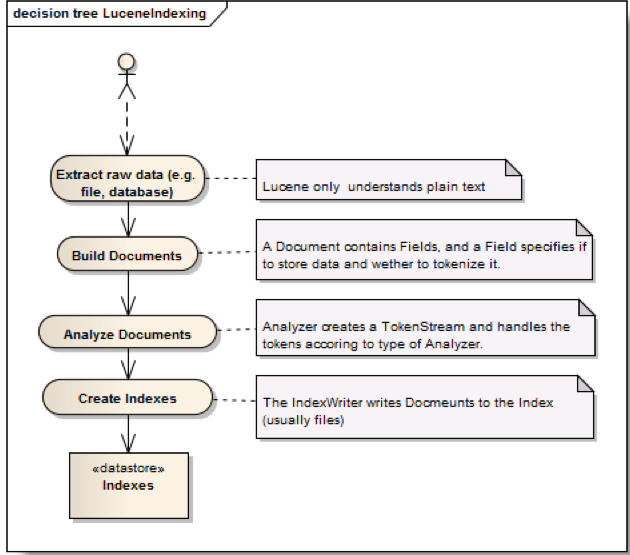
\includegraphics[scale=0.5]{images/decision_tree_luceneindexing.png}
	\caption{The indexing "pipeline" \protect\footnotemark}
	\label{xkcd_standards_fig}
\end{figure}
\footnotetext{Footnote für Bild}

\paragraph{Usage}
Using Lucene as a standalone engine requires the programmer to design the engine from the bottom up. The developer has to write all the logic, starting with the actual indexing code through to the code managing access to the index. The conversion from Java objects to Documents (for indexing) and back (for searching) have to be implemented as well. This whole process requires a lot of code to be written and the API only helps by providing the necessary tools. This has one additional problem: The Lucene API tends to change a lot between versions and the code has to be kept up-to-date. It's not uncommon that whole features that were state-of-the-art in one version, are deprecated (potentially unstable, marked to be removed in the future) in the next release, resulting in big code changes being potentially necessary.

\paragraph{Features}
Lucene probably is the most complete toolbox to build a search-engine from. It has pre-built analyzers for many languages, a queryparser to support generating queries out of user input, a phonetic module, a faceting module, and many other features. While mostly known for its fulltext capabilities, it also has modules used for other purposes, for example the spatial module that enables geo-location query support.

\subsubsection{Solr}

\begin{quote}
	Solr is the popular, blazing-fast, open source enterprise search platform built on Apache Lucene™.
\end{quote}

\subsubsection{ElasticSearch}

\subsubsection{Hibernate Search}

\begin{quote}
Hibernate Search transparently indexes your objects and offers fast regular, full-text and geolocation search. Ease of use and easy clustering are core.\footnote{Hibernate Search project homepage, see~\cite{hibernate_search_homepage}}
\end{quote}

\textcolor{red}{some kind of conclusion with a table of features. -> Hibernate Search, aber mit dem Problem von Kompatibilität mit Non Hibernate ORM, mention Compass?}

\subsubsection{Conclusion: Why a generic Hibernate Search?}

\subsection{Versions used in this Thesis}

\textcolor{red}{Hier die Versionen, die benutzt werden auflisten für Hibernate Search, Hibernate ORM, EclipseLink, OpenJPA}

\pagebreak